\documentclass{report}
\usepackage{geometry}
\usepackage{paralist}
\usepackage{scalerel,amssymb}
\usepackage{tikz}
\usepackage{amsmath}
\usepackage{array}
\usepackage{nccmath}
\usepackage{pgfplots}

\usepackage{fancyhdr}
\fancyhead[L]{\LARGE Applied Optimization \\
\Large Exercise 05}
\fancyhead[R]{13-123-922 \\
Elias \textsc{Wipfli} \\
13-933-262 \\
Lorenzo \textsc{Wipfli} \\
16-124-836 \\
Marcel \textsc{Zauder}}
\renewcommand{\headrulewidth}{0.4pt}
\fancyfoot[C]{\thepage}
\renewcommand{\footrulewidth}{0.4pt}

\definecolor{darkgreen}{rgb}{0.0, 0.4, 0.0}

\usepackage{hyperref}

\begin{document}
	\pagestyle{fancy}
	\hfill \\ \\
	
	\section*{5.1 Exact line search for the convex quadratic function}
	\section*{5.2 Gradient descent with exact line search}
	\begin{enumerate}[]
		\item Given properties:
		\begin{enumerate}[(i)]
			\item \textbf{objective function:} $f(x) \ = \ \frac{1}{4} x_1^2 + x_2^2$
			\item \textbf{starting point:} $x^{(0)} \ = \ (2,1)$
		\end{enumerate}
		With this we can calculate the following:
		\begin{align*}
			& & \bigtriangledown f(x) \ & = \ \left(\begin{array}{c} \frac{1}{2} x_1 \\ 2 x_2 \end{array}\right) \\
			& \Rightarrow & \ \bigtriangledown f(x^{(0)}) \ & = \ \left(\begin{array}{c} \frac{1}{2} \cdot 2 \\ 2 \cdot 1 \end{array}\right) \  = \ \left(\begin{array}{c} 1 \\ 2 \end{array}\right) \ =: \ \Delta x \\
			& \Rightarrow & \ x^{(1)} \ & := \ x^{(0)}  + t \Delta x \\
			& & & = \ \left(\begin{array}{c} 2 \\ 1 \end{array}\right) + t \cdot \left(\begin{array}{c} 1 \\ 2 \end{array}\right) \\
			& & & = \ \left(\begin{array}{c} 2+t \\ 1+2t \end{array}\right) \\
			& \Rightarrow & \ \| \bigtriangledown f(x^{(1)} \| _2 \ = \ \| \left(\begin{array}{c} 2+t \\ 1+2t \end{array}\right) \| _2 \ & = \ \sqrt{(1+\frac{1}{2}t)^2 + (2+4t)^2} \\
			& & & = \ \sqrt{1+t+\frac{1}{4}t^2 + 4 + 8t + 16t^2} \\
			& & & = \ \sqrt{5 + 9t + \frac{65}{4}t^2}
		\end{align*}
		
		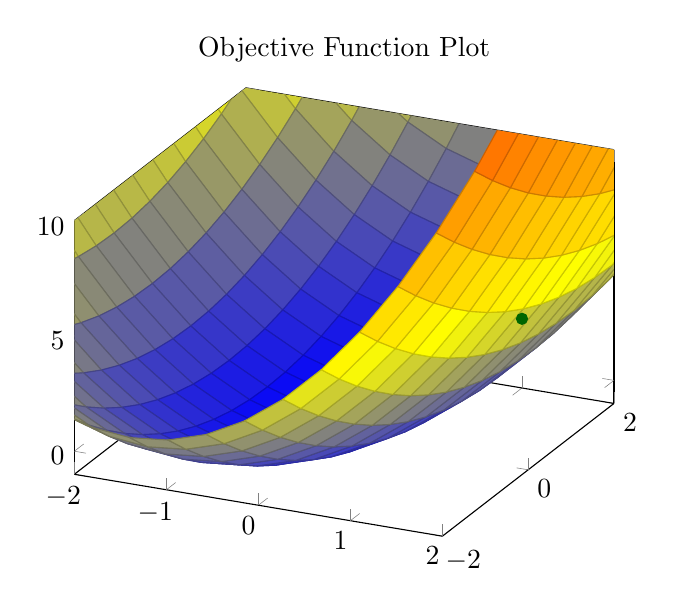
\begin{tikzpicture}
	        \begin{axis}[
	            title={Objective Function Plot},
	            xmin = -2, xmax = 2, ymin = -2, ymax = 2, zmin = -1, zmax = 10,
	    ]
	    		%Functions
	            \addplot3[surf]{0.25*y^2 + x^2};
	            
	            %Nodes
	            \addplot3[mark=*, color=darkgreen] coordinates {(1,2,2)};            
	            
	        \end{axis}
	    \end{tikzpicture}
		
	\end{enumerate}
	\section*{5.3 Programming Exercise: Constrained Mass Spring System}
		
\end{document}